\begin{center}
\begin{tikzpicture}
\begin{axis}[
    width=\dimexpr0.5\linewidth-1cm\relax,
    height=\dimexpr0.5\linewidth-1cm\relax,
    grid=both,
    unbounded coords=jump,
    title style={font=\small, yshift=0.6em},
    xlabel=$t$,
    ylabel style={%
        rotate=-90,
        anchor=east,
        overlay%
    },
    ylabel={$\varphi(t)=\dfrac{1+\tfrac{1}{2} e^{2t}}{1-\tfrac{1}{2} e^{2t}}$},
    xmin=-1.2, xmax=1.2,
    ymin=-10, ymax=10,
    % title={$\varphi(t)=\dfrac{1+\tfrac12 e^{2t}}{1-\tfrac12 e^{2t}}$},
]
\pgfmathsetmacro{\asymp}{0.5*ln(2)}
\addplot[dashed,gray,domain=-1.2:1.2]{1};
\addplot[dashed,gray,samples=2] coordinates {(\asymp,-10) (\asymp,10)} node[pos=0.9,right] {$\frac{1}{2}\ln(2)$};
\addplot[blue,thick,domain=-1.2:\asymp,samples=200,restrict y to domain=-10:10]
  {(1 + 0.5*exp(2*x)) / (1 - 0.5*exp(2*x))};
\addplot[gray,thick,domain=\asymp+0.002:1.2,samples=200,restrict y to domain=-10:10]
  {(1 + 0.5*exp(2*x)) / (1 - 0.5*exp(2*x))};
\addplot[only marks, mark=*, mark size=1.5pt, blue] coordinates {(0,3)};
\node[blue] at (axis cs:-0.25,3.5) {$(0,3)$};
\end{axis}
\end{tikzpicture}
\end{center}